\documentclass[12pt]{article}

\usepackage[english]{babel}
\usepackage[utf8]{inputenc}
\usepackage{sansmathfonts}
\usepackage[T1]{fontenc}
\renewcommand*\familydefault{\sfdefault} %% Only if the base font of the document is to be sans serif
\usepackage{multicol,lipsum}
\usepackage{amsmath,cancel}
\usepackage{amssymb,amsthm,dsfont,mathrsfs}
\usepackage[colorinlistoftodos]{todonotes}
\usepackage{geometry}
\geometry{
a4paper,
total={170mm,257mm},
left=20mm,
top=15mm,
bottom=22mm,
}
\usepackage{natbib}
\usepackage{soul}
\usepackage{setspace}
\usepackage{hyperref}
\usepackage{xcolor}
\usepackage{graphicx}
\usepackage{tikz}
\usepackage{siunitx}
\graphicspath{ {imagens/} }
\usepackage{fancyhdr}
\pagestyle{fancy}
\renewcommand{\headrulewidth}{0pt}

\color{darkgray}
\newcommand{\T}[1]{\vspace{0.4cm}\textbf{\large#1}}
\newcommand{\TW}[1]{\textbf{\large#1}}

\newcommand{\TM}[1]{\vspace{0.2cm} \textbf{#1}}

\newcommand{\M}[1]{
\vspace{-0.6cm}
\begin{flalign*}
#1&
\end{flalign*}
\vspace{-0.6cm}
}


\definecolor{bluebell}{rgb}{0.25, 0.35, 0.89} 
\definecolor{laranja}{rgb}{0.87, 0.48, 0.25} 
\definecolor{verde}{rgb}{0, 0.54, 0.44} 
\definecolor{babypink}{rgb}{1, 0.42, 0.52} 
\definecolor{rosa}{rgb}{1, 0.72, 0.77} 
\definecolor{cinza}{rgb}{0.3, 0.3, 0.3}  
\definecolor{iris}{rgb}{0.25, 0.35, 0.89}  
\definecolor{babyblue}{rgb}{0.13, 0.59, 0.95}

\setlength\columnsep{30pt}

\setlength{\parindent}{0cm}
\setlength{\fboxrule}{1.3pt}  % <-- Aumenta a espessura

\newcommand{\Formula}[1]{
\begin{center}
\color{iris}
\fcolorbox{rosa}{white}{
\(
\begin{array}{c}
#1
\end{array}
\)
}
\color{cinza}
\end{center}
}

\begin{document}
\pagenumbering{gobble}
\setstretch{1.3}


\includegraphics[width=4cm]{Logo2.png}
\begin{center}
    \textbf{\Huge \textcolor{bluebell}{Funções Trigonométricas}}
\end{center}

\begin{multicols}{2}

% ── RADIANO ────────────────────────────────────────────────────────────────
\TW{Radiano}

Um \textbf{radiano} é o ângulo central que intercepta um arco de comprimento igual ao raio.
Como a volta completa tem comprimento $2\pi r$:

\Formula{\pi\;\text{rad} = 180° \qquad 1\;\text{rad} \approx 57{,}3°}

\TM{Conversão grau $\leftrightarrow$ radiano:}

\Formula{\text{rad} = \text{grau} \times \dfrac{\pi}{180} \qquad \text{grau} = \text{rad} \times \dfrac{180}{\pi}}

\TM{Arcos notáveis:}

$30° = \dfrac{\pi}{6}$ \quad $45° = \dfrac{\pi}{4}$ \quad $60° = \dfrac{\pi}{3}$

$90° = \dfrac{\pi}{2}$ \quad $180° = \pi$ \quad $270° = \dfrac{3\pi}{2}$ \quad $360° = 2\pi$

\TM{Exemplos de conversão:}

$135° = 135 \times \dfrac{\pi}{180} = \dfrac{3\pi}{4}$ rad

$\dfrac{5\pi}{6} \times \dfrac{180}{\pi} = 150°$

% ── CICLO TRIGONOMÉTRICO ───────────────────────────────────────────────────
\TW{Ciclo Trigonométrico}

Circunferência de raio 1. Para ângulo $\theta$, o ponto $P$ sobre o ciclo tem:

\Formula{P = (\cos\theta,\; \operatorname{sen}\theta)}

\begin{center}
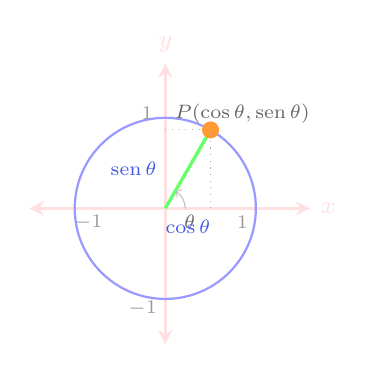
\begin{tikzpicture}[scale=1.15]
\tikzstyle{eixo}=[pink!50!white, line width=1.3pt]
\draw[eixo, stealth-stealth] (-1.5,0) -- (1.6,0) node[right, font=\small] {$x$};
\draw[eixo, stealth-stealth] (0,-1.5) -- (0,1.6) node[above, font=\small] {$y$};
\draw[blue!40!white, thick] (0,0) circle (1);
\draw[green!60!white, line width=1.2pt] (0,0) -- ({cos(60)},{sin(60)});
\filldraw[orange!80!white] ({cos(60)},{sin(60)}) circle (2.5pt);
\node[black!60!white, font=\scriptsize] at (0.85,1.05) {$P(\cos\theta,\operatorname{sen}\theta)$};
\draw[dotted, gray!60!white] ({cos(60)},0) -- ({cos(60)},{sin(60)});
\draw[dotted, gray!60!white] (0,{sin(60)}) -- ({cos(60)},{sin(60)});
\node[font=\scriptsize, black!60!white] at (0.27,-0.15) {$\theta$};
\draw[gray!50!white, ->] (0.22,0) arc (0:60:0.22);
\node[font=\scriptsize, iris] at ({cos(60)/2},-0.2) {$\cos\theta$};
\node[font=\scriptsize, iris] at (-0.35,{sin(60)/2}) {$\operatorname{sen}\theta$};
\node[font=\scriptsize, black!40!white] at (0.85,-0.15) {$1$};
\node[font=\scriptsize, black!40!white] at (-0.85,-0.15) {$-1$};
\node[font=\scriptsize, black!40!white] at (-0.2,1.05) {$1$};
\node[font=\scriptsize, black!40!white] at (-0.25,-1.1) {$-1$};
\end{tikzpicture}
\end{center}

Sinais por quadrante:

1º Q: sen $> 0$ e cos $> 0$ \quad 2º Q: sen $> 0$ e cos $< 0$

3º Q: sen $< 0$ e cos $< 0$ \quad 4º Q: sen $< 0$ e cos $> 0$

% ── TABELA DE VALORES NOTÁVEIS ─────────────────────────────────────────────
\TW{Valores Notáveis}

\vspace{0.2cm}
\begin{center}
\renewcommand{\arraystretch}{1.35}
\setlength{\tabcolsep}{4pt}
{\small
\begin{tabular}{|c|c|c|c|c|c|}
\hline
 & $0°$ & $30°$ & $45°$ & $60°$ & $90°$ \\
\hline
\textbf{sen} & $0$ & $\tfrac{1}{2}$ & $\tfrac{\sqrt{2}}{2}$ & $\tfrac{\sqrt{3}}{2}$ & $1$ \\
\hline
\textbf{cos} & $1$ & $\tfrac{\sqrt{3}}{2}$ & $\tfrac{\sqrt{2}}{2}$ & $\tfrac{1}{2}$ & $0$ \\
\hline
\textbf{tg} & $0$ & $\tfrac{\sqrt{3}}{3}$ & $1$ & $\sqrt{3}$ & $\nexists$ \\
\hline
\end{tabular}
}
\end{center}

Para $180°$: sen $= 0$, cos $= -1$, tg $= 0$.

Para $270°$: sen $= -1$, cos $= 0$, tg $= \nexists$.

\fcolorbox{laranja}{white}{\parbox{0.85\linewidth}{
\small\textbf{Macete para o seno:}
$0° \to \tfrac{\sqrt{0}}{2}$, \; $30° \to \tfrac{\sqrt{1}}{2}$, \; $45° \to \tfrac{\sqrt{2}}{2}$,
\; $60° \to \tfrac{\sqrt{3}}{2}$, \; $90° \to \tfrac{\sqrt{4}}{2} = 1$.
O cosseno segue o padrão invertido.
}}

% ── GRÁFICOS DE SENO E COSSENO ─────────────────────────────────────────────
\TW{Gráficos de Seno e Cosseno}

Ambas as funções são \textbf{periódicas} com período $2\pi$, amplitude 1,
domínio $\mathbb{R}$ e imagem $[-1, 1]$.

\begin{center}
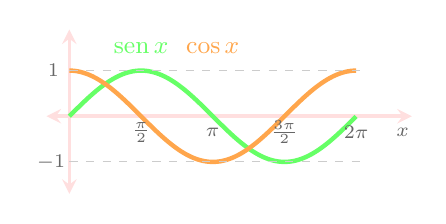
\begin{tikzpicture}[scale=0.58]
\tikzstyle{eixo}=[pink!50!white, line width=1.3pt]
\draw[eixo, stealth-stealth] (-0.5,0) -- (7.5,0);
\draw[eixo, stealth-stealth] (0,-1.7) -- (0,1.9);
\draw[green!60!white, line width=1.6pt, domain=0:6.28, samples=100]
    plot (\x, {sin(\x r)});
\draw[orange!70!white, line width=1.6pt, domain=0:6.28, samples=100]
    plot (\x, {cos(\x r)});
\node[green!60!white, font=\small]  at (1.57,1.5) {$\operatorname{sen} x$};
\node[orange!70!white, font=\small] at (3.14,1.5) {$\cos x$};
\draw[dashed, gray!40!white] (0,1) -- (6.5,1);
\draw[dashed, gray!40!white] (0,-1) -- (6.5,-1);
\node[font=\scriptsize, black!60!white] at (-0.35,1) {$1$};
\node[font=\scriptsize, black!60!white] at (-0.4,-1) {$-1$};
\node[font=\scriptsize, black!60!white] at (1.57,-0.35) {$\tfrac{\pi}{2}$};
\node[font=\scriptsize, black!60!white] at (3.14,-0.35) {$\pi$};
\node[font=\scriptsize, black!60!white] at (4.71,-0.35) {$\tfrac{3\pi}{2}$};
\node[font=\scriptsize, black!60!white] at (6.28,-0.35) {$2\pi$};
\node[font=\scriptsize, black!60!white] at (7.3,-0.35) {$x$};
\end{tikzpicture}
\end{center}

Seno: zeros em $x = k\pi$ ($k \in \mathbb{Z}$).

Cosseno: zeros em $x = \dfrac{\pi}{2} + k\pi$ ($k \in \mathbb{Z}$).

$\cos x = \operatorname{sen}\!\left(x + \dfrac{\pi}{2}\right)$ — cosseno é seno deslocado.

% ── TANGENTE ───────────────────────────────────────────────────────────────
\TW{Função Tangente}

\Formula{\operatorname{tg} x = \dfrac{\operatorname{sen} x}{\cos x}}

Não definida quando $\cos x = 0$, ou seja, em $x = \dfrac{\pi}{2} + k\pi$.

Domínio: $\mathbb{R} \setminus \!\left\{\dfrac{\pi}{2} + k\pi,\; k \in \mathbb{Z}\right\}$

Imagem: $\mathbb{R}$ \quad Período: $\pi$ \quad Crescente em cada intervalo do domínio.

$\operatorname{tg} 30° = \tfrac{\sqrt{3}}{3}$ \quad $\operatorname{tg} 45° = 1$ \quad $\operatorname{tg} 60° = \sqrt{3}$

% ── IDENTIDADES ────────────────────────────────────────────────────────────
\TW{Identidades Trigonométricas}

Do Teorema de Pitágoras no círculo unitário (hipotenusa = 1):

\Formula{\operatorname{sen}^2 x + \cos^2 x = 1}

\TM{Identidades derivadas:}

Dividindo por $\cos^2 x$: \quad $\operatorname{tg}^2 x + 1 = \sec^2 x$

Dividindo por $\operatorname{sen}^2 x$: \quad $1 + \operatorname{cotg}^2 x = \csc^2 x$

\TM{Exemplo — calcule $\cos x$ dado $\operatorname{sen} x = \tfrac{3}{5}$ no 1º quadrante:}

$\dfrac{9}{25} + \cos^2 x = 1 \;\Rightarrow\; \cos^2 x = \dfrac{16}{25}$

$\cos x = \dfrac{4}{5}$ \hfill {\small(positivo no 1º quadrante)}

\TM{Ângulos especiais:}

$\operatorname{sen}(180° - \theta) = \operatorname{sen}\theta$ \quad $\cos(180° - \theta) = -\cos\theta$

$\operatorname{sen}(-\theta) = -\operatorname{sen}\theta$ \quad $\cos(-\theta) = \cos\theta$

\end{multicols}

\lfoot{\scriptsize © Copyright, Pratique Já}
\cfoot{\large \textcolor{bluebell}{pratiqueja.com}}
\end{document}
